% Chapter 1
\chapter{Introduction} % Main chapter title
\label{Chapter1} % For referencing the chapter elsewhere, use \ref{Chapter1} 
\lhead{Chapter 1. \emph{Introduction}} % This is for the header on each page - perhaps a shortened title
%----------------------------------------------------------------------------------------

\par This is general template for those wizards, who rose above and beyond Word. From now on, they can manipulate the reality and matter with new so advanced tool \LaTeX{}.

\par  Blown Away By Magic!

%----------------------------------------------------------------------------------------
\section{Motivation}
%----------------------------------------------------------------------------------------

\par 

\par 

\par 

%----------------------------------------------------------------------------------------
\subsection{Abstract}
%----------------------------------------------------------------------------------------

\par Figure \ref{fig:phd-abstract.png} see more \href{https://phdcomics.com/comics/archive_print.php?comicid=1121}{in}.
% https://phdcomics.com/comics/archive_print.php?comicid=1121

\begin{figure}[H]
    \centering
    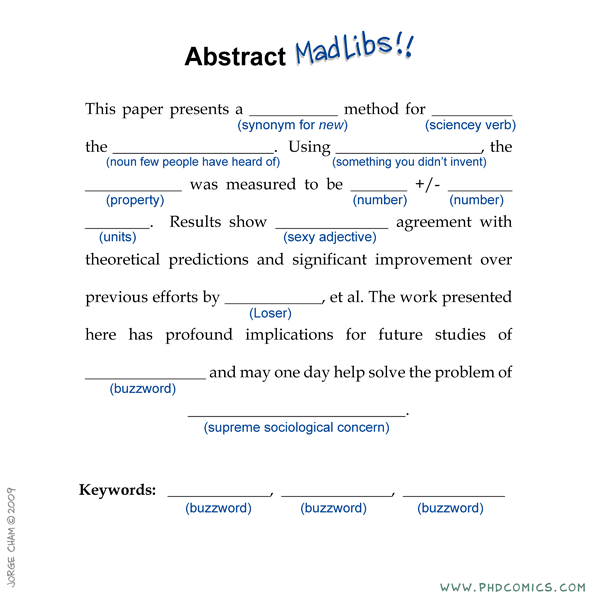
\includegraphics[scale=0.9]{Figures/phd-abstract.png}
    %\rule{35em}{0.5pt}
    \caption[Abstract]{\href{https://phdcomics.com/comics/archive_print.php?comicid=1121}{Abstract}}
    \label{fig:phd-abstract.png}
\end{figure}

%----------------------------------------------------------------------------------------
\subsection{Outline}
%----------------------------------------------------------------------------------------

\par Look other your outline Figure \ref{fig:phd-outline.png} see more \href{http://phdcomics.com/comics/archive.php?comicid=715}{link}.
% http://phdcomics.com/comics/archive.php?comicid=715

\begin{figure}[H]
    \centering
    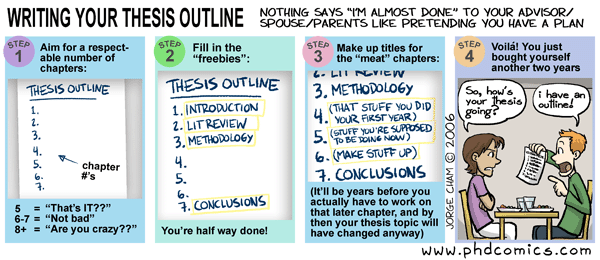
\includegraphics[scale=0.9]{Figures/phd-outline.png}
    %\rule{35em}{0.5pt}
    \caption[Outline]{\href{http://phdcomics.com/comics/archive.php?comicid=715}{Outline}}
    \label{fig:phd-outline.png}
\end{figure}

%----------------------------------------------------------------------------------------
\section{Background}
%----------------------------------------------------------------------------------------



\par 

\par 

%----------------------------------------------------------------------------------------
\subsection{Typical Structure of a Thesis}
%----------------------------------------------------------------------------------------

\begin{itemize}
    \item Title Page (Figure \ref{fig:phd-title.png})
    \item Specific title of the thesis (e.g. “Multi-stage Learning in Biomimetic Search and Rescue Robots”)
    \item General Title (i.e. “Final Year Project Report”)
\begin{figure}[H]
    \centering
    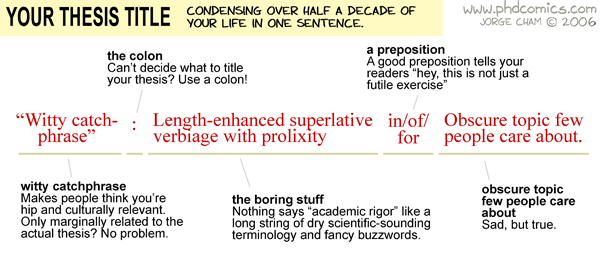
\includegraphics[scale=0.9]{Figures/phd-title.png}
    %\rule{35em}{0.5pt}
    \caption[Title]{\href{http://phdcomics.com/comics/archive_print.php?comicid=718}{Title}}
    \label{fig:phd-title.png}
\end{figure}

    \item Degree (e.g. Ph.D., M.Sc., B. Sc.)
    \item Author (name and student identification number)
    \item Institution 
    \item Supervisor
    \item Date
    \item Table of Contents
    \item Chapters
    \item Sections
    \item Acknowledgements (Help from friends, colleagues, and staff. Support from sponsor... Support from Parents, etc... )
     \item Chapter 1. Introduction & Overview
    \item Chapter 2. Literature Survey
    \item Chapter 3. Theoretical Foundations: Background Material
    \item Chapter 4. Formal Model: Theoretical Development (use additional chapters if necessary)
    \item Chapter 5. Algorithmic Considerations
    \item Chapter 6. Implementation Issues
    \item Chapter 7. Evaluation
    \item Chapter 8. Discussion and Critical Appraisal
    \item References
    \item Appendices
    \item Key Software listings, Code, Diagrams
    \item Mechanical schematics
    \item Mathematical proofs
\end{itemize}

%----------------------------------------------------------------------------------------
\subsection{Items}
%----------------------------------------------------------------------------------------

\par 

\begin{enumerate}
    \item One 
    \item Two
    \item 
    \item 
    \item 
    \item 
    \item 
\end{enumerate}

\begin{itemize}
    \item 1
    \item 2
    \item 
    \item 
    \item 
    \item 
    \item 
    \item 
\end{itemize}

\par 

\par 

%----------------------------------------------------------------------------------------
\section{Problem}
%----------------------------------------------------------------------------------------

\par 

%----------------------------------------------------------------------------------------
\section{Goals}
%----------------------------------------------------------------------------------------

\par 

%----------------------------------------------------------------------------------------
\section{Objectives}
%----------------------------------------------------------------------------------------

\par 

%----------------------------------------------------------------------------------------
\section{Contributions}
%----------------------------------------------------------------------------------------

\par 

%----------------------------------------------------------------------------------------
\section{Future goals}
%----------------------------------------------------------------------------------------

\par 

\par 

%----------------------------------------------------------------------------------------
\section{Outline}
%----------------------------------------------------------------------------------------

\par We will preside this thesis in a following structure \cite{David-Vernon}, \cite{David-Vernon1}:
\begin{itemize}
\item Chapter 1: Introduction, Background, Motivation, Problem statement, Goals, Restrictions, Overview;
\item Chapter 2: Literature Survey and Background:  Research method, Methodology of Software Development, Literature review, Related Works
\item Chapter 3: Theoretical Foundations: Background Material, State of art, Theory on hardware, Architecture
\item Chapter 4: Protocol and systems(services and programs) used to build the system.
\item Chapter 5: Formal Model: Theoretical Development, Implementation / Use cases, Testing
\item Chapter 6: Algorithmic Considerations
\item Chapter 7: Implementation Issues, Results and Evaluation
\item Chapter 8: Discussion, Critical Appraisal, Conclusions
\item Chapter 9: Future Work 
\end{itemize}

%Chapter 1. Introduction & Overview
%Chapter 2. Literature Survey
%Chapter 3. Theoretical Foundations: Background Material
%Chapter 4. Formal Model: Theoretical Development (use additional chapters if necessary)
%Chapter 5. Algorithmic Considerations
%Chapter 6. Implementation Issues
%Chapter 7. Evaluation
%Chapter 8. Discussion & Critical Appraisal
%References
%Appendices
% Key Software listings
% Mechanical schematics
% Mathematical proofs
%----------------------------------------------------------------------------------------
%----------------------------------------------------------------------------------------


%Typical Structure of a Thesis
%Title Page
% Specific title of the thesis (e.g. “Multi-stage Learning in Biomimetic Search and Rescue Robots”)
% General Title (i.e. “Final Year Project Report”)
%% Degree (e.g. Ph.D., M.Sc., B. Sc.)
% Author (name and student identification number)
% Institution (i.e. University of Skövde)
% Supervisor
% Date
%Abstract
% What is the subject matter of the thesis: what did you do?
% Motivation: why is it important?
% Significance: what contribution does the thesis make?
% The abstract should be approximately 200 words long. It normally takes at least ten revisions to achieve a good abstract.
% The abstract should be written after the thesis has been completed.
%Table of Contents
% Chapters
% Sections
%Acknowledgements
% Help from friends, colleagues, and staff.
% Support from sponsor
% Support from Parents, etc
%Chapter 1. Introduction & Overview
%Chapter 2. Literature Survey
%Chapter 3. Theoretical Foundations: Background Material
%Chapter 4. Formal Model: Theoretical Development (use additional chapters if necessary)
%Chapter 5. Algorithmic Considerations
%Chapter 6. Implementation Issues
%Chapter 7. Evaluation
%Chapter 8. Discussion & Critical Appraisal
%References
%Appendices
% Key Software listings
% Mechanical schematics
% Mathematical proofs
